The BJT is comprised of a linear array of three layers of extrinsic semiconductor materials with alternating types (NPN or PNP). The following figure aids with visualization of the physical structure of the BJT:

\FloatBarrier

\begin{figure}[h!]
	\centering
	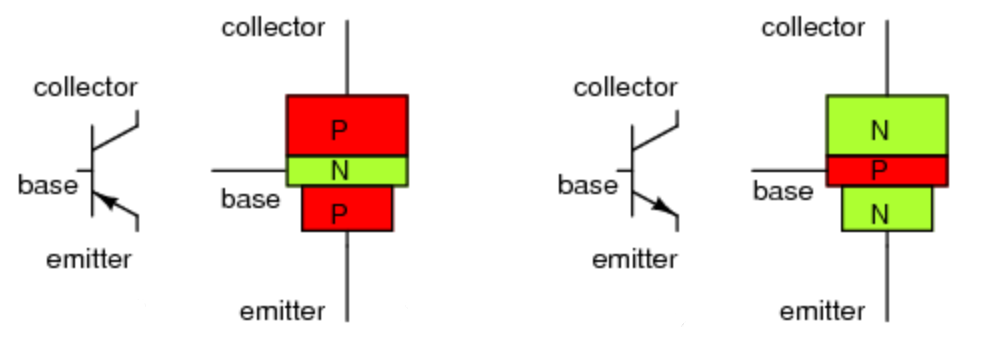
\includegraphics[scale=0.75]{./images/bjt_fig.PNG}
	\caption{Schematic Symbol and Structure of PNP and NPN BJT}
	\label{fig:id_vs_vgs}
\end{figure}

\FloatBarrier

The three layers of semiconductor material form regions called the emitter, base, and collector. The three regions essentially form two semiconductor junctions that share a common thin base region. The emitter region has a significantly higher doping concentration than the other regions. 

Charge generated in the BJT is caused by the diffusion of majority carriers from the emitter to base region. The charge carriers that passed from the emitter to the base are now the excess minority carriers of the region and they diffuse to the collector region due to the thin physical length of the base, which is assumed to be the same order of magnitude of the width of the depletion regions of the semiconductor junctions in the BJT. The thinness of the base layer is crucial so that carriers can diffuse across it much faster than the minority carrier lifetime of the base semiconductor material to prevent loss due to recombination. For a PNP BJT, holes from the p-type emitter diffuse to the n-type base and then diffuse to the p-type collector to generate the collector current across the BJT. For an NPN BJT, electrons from the n-type emitter diffuse to the p-type base and then diffuse to the n-type collector to generate the collector current across the BJT.  In this experiment, an NPN BJT, model MPSA06, is analyzed.

The charge generated by the  NPN BJT is propagated by a forward bias applied across the base-emitter junction ($V_{BE}$) and a reverse bias applied across the base-collector junction ($V_{CE}$). For majority charge carriers (electrons) to overcome the depletion region at the base-emitter junction, a sufficiently large $V_{BE}$ must be applied. At voltage values that are less than that threshold, the carriers cannot overcome the energy barrier at the depletion zone, and therefore the carrier current, $I_C$, is zero. This is referred to as the cut-off region. When the $V_{BE}$ is above the threshold value, the energy barrier is lowered so that the electrons can diffuse from the emitter to base, thus turning on the junction. After the threshold value is met, increase in $V_{BE}$ causes an exponential increase in $I_C$, much like the I-V behavior of a pn-junction diode.

\FloatBarrier

\begin{figure}[h!]
	\centering
	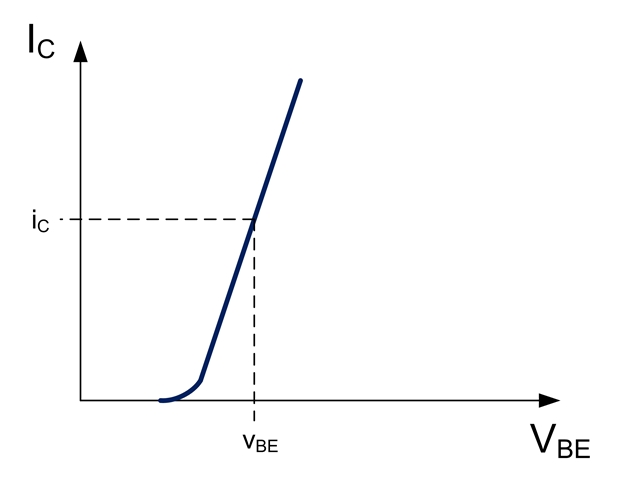
\includegraphics[scale=3]{./images/bjt_ic_vbe_expected.PNG}
	\caption{Expected $I_C$ versus $V_{BE}$ Curve for a NPN BJT}
	\label{fig:ic_vs_vbe}
\end{figure}

\FloatBarrier

After the electrons from the emitter region diffuse to the base region, a sufficiently large voltage must be applied across the base-collector junction for the electrons to then diffuse from the base to the collector region. This voltage is referred to as $V_C$ which is the same as $V_{CE}$ because the emitter in our experimental schematic is grounded. A linear increase in $I_C$ is expected for values of $V_{CE}$ that are less than the amount of voltage in which $V_{BE}$ has overtaken the threshold voltage. As $V_{CE}$ continues to increase, the base region loses so many electrons that the conductivity of the base drops which effectively limits the increase in $I_C$ and $I_C$ is expected to reach a constant maximum beyond that threshold value. The region in which $I_C$ increases linearly is referred to as the saturation region, as the biasing polarity of the collector-base junction is reversed when $V_{CE}$ is lower than the threshold voltage value explained above. Increasing $V_{BE}$ causes $I_C$ to saturate at a larger current value.

\FloatBarrier

\begin{figure}[h!]
	\centering
	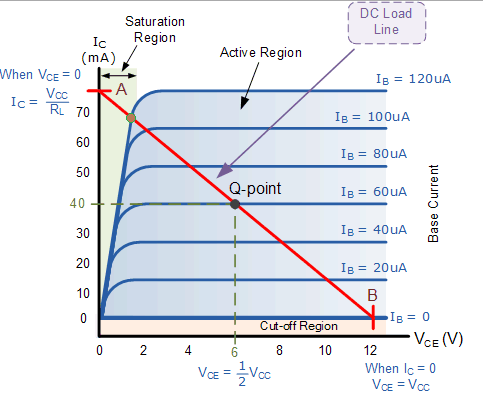
\includegraphics[scale=0.75]{./images/bjt_ic_vce_expected.PNG}
	\caption{Expected $I_C$ versus $V_{E}$ Curve for a NPN BJT}
	\label{fig:ic_vs_vce}
\end{figure}

\FloatBarrier

The following circuit is used to measure and analyze the $I_C - V_{BE}$ and $I_C - V_{CE}$ curves:


\FloatBarrier

\begin{figure}[h!]
	\centering
	\caption{BJT Measurement Circuit}
	\label{fig:bjt_circ}
	\begin{circuitikz}
		\draw
		( 0 , 0 ) node[ npn ] (my_npn) {}
		(my_npn.B) to [ R ] ++( -2 , 0 ) coordinate(r_in)
		(my_npn.B) node[label={ [font=\normalsize] above : $V_{BE}$ } ] { }
		(r_in) to [ battery , v<=$V_1$ ] ++( 0 , -2 ) coordinate(gnd_1)
		(gnd_1) node[ ground ] (my_gnd_1) {}
		(my_npn.E) node[ ground ] (my_gnd_2) {}
		(my_npn.C) to [ R , i<_=$I_C$] ++( 0 , 2 ) coordinate(r_c)
		(my_npn.C) node[label={ [font=\normalsize] below : $V_{CE}$ } ] { }
		(r_c) to [ battery , v<=$V_2$ ] ++( 2 , 0 ) coordinate(gnd_3)
		(gnd_3) node[ ground ] (my_gnd_3) {}
		;
	\end{circuitikz}
\end{figure}

\FloatBarrier

The $I_C - V_{BE}$ plot is measured by fixing $V_2$ at 5V and sweeping $V_1$ from 0V to 5V. $V_{BE}$ is measured by probing the base lead to the emitter lead (ground) of the BJT. The voltage across the resistor connected to the collector lead of the BJT is also probed so that $I_C$ can be calculated from the voltages measured by the probe. $I_C$ has a simple Ohmic relationship with the voltage across the resistor connected to the collector lead. The following values are tabulated following the configuration as described above:

\FloatBarrier

\begin{table}[h!]
	\centering
	\caption{BJT $I_C$ versus $V_{BE}$ Data}
	\label{tab:bjt_ic_vbe}
	\csvautotabular{./tables/bjt_ic_vbe.csv}
\end{table}

\FloatBarrier

{\footnotesize $I_C$ has an Ohmic relationship with the voltage across the resistor connected to the collector, thus $I_C$ is calculated using Ohm's law. The resistor connected to the collector is measured to be 0.998\si{\kilo\ohm} and the resistor connected to the base is 9.902\si{\kilo\ohm}. $V_2$ is fixed to $5$\si{\volt}.}

\FloatBarrier

Subsequently, the following plot is generated from the values in Table \ref{tab:bjt_ic_vbe}:

\begin{figure}[h!]
	\centering
	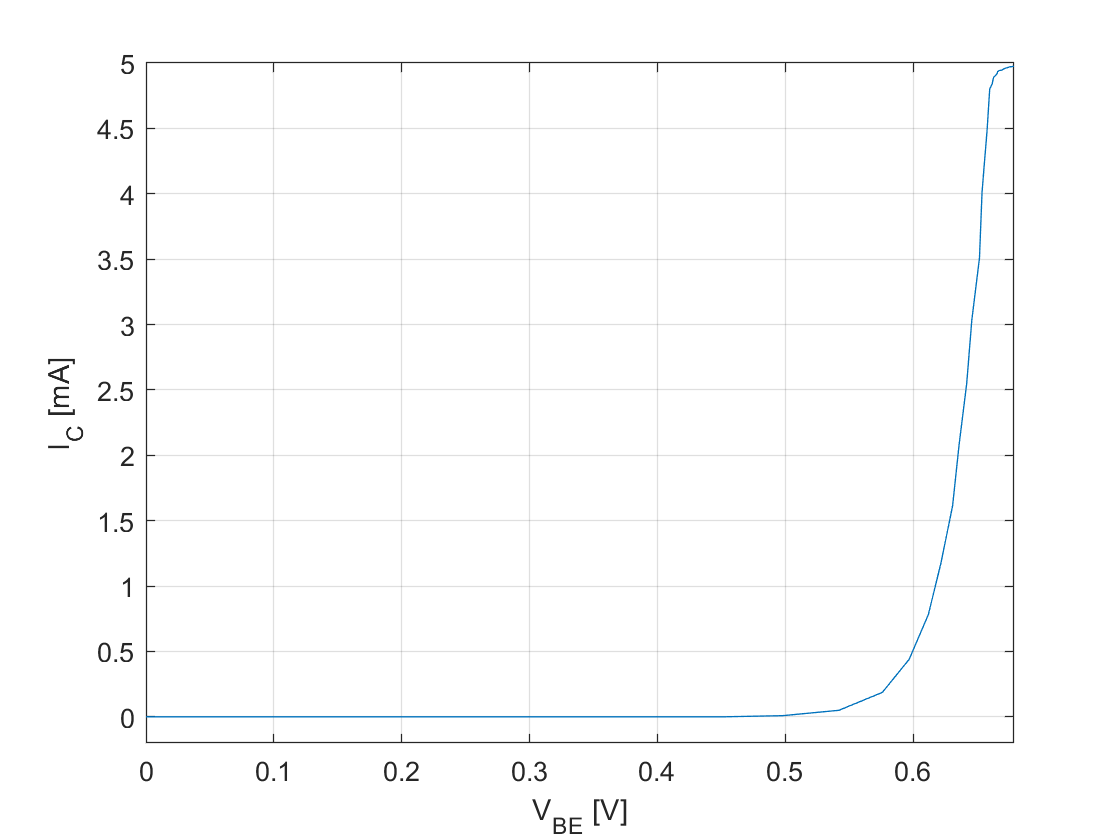
\includegraphics[scale=0.4]{./images/bjt_ic_vbe.PNG}
	\caption{BJT $I_C$ versus $V_{BE}$ Plot}
	\label{fig:bjt_ic_vbe}
\end{figure}

\FloatBarrier

The $I_C - V_{BE}$ curve from the measured values above exhibit the expected behavior. The BJT is observed to turn on when $V_{BE}$ reaches approximately 0.6V. This is consistent with the turn-on voltage of a typical pn-junction diode, which shares its physical composition with the base-emitter junction of the BJT. The curve is then observed to flatten when the $V_{BE}$ becomes closer to $V_{CE}$ as the saturation bias configuration is reached.

The $I_C - V_{CE}$ plot is measured by fixing $V_1$ at 1V and sweeping $V_2$ from 0V to 10V. $V_{CE}$ is measured by probing the collector lead to the emitter lead (ground) of the BJT. The voltage across the resistor connected to the collector lead of the BJT is again probed so that $I_C$ can be calculated from the voltages measured by the probe like before in the previous measuring configuration. The following values are tabulated following the configuration as described above:

\FloatBarrier

\begin{table}[h!]
	\centering
	\caption{BJT $I_C$ versus $V_{CE}$ Data}
	\label{tab:bjt_ic_vce}
	\csvautotabular{./tables/bjt_ic_vce.csv}
	\\
	(\footnotesize $V_1$ is fixed at $1$\si{\volt}.)
\end{table}



\FloatBarrier

Subsequently, the following plot is generated from the values in Table \ref{tab:bjt_ic_vce}:

\FloatBarrier

\begin{figure}[h!]
	\centering
	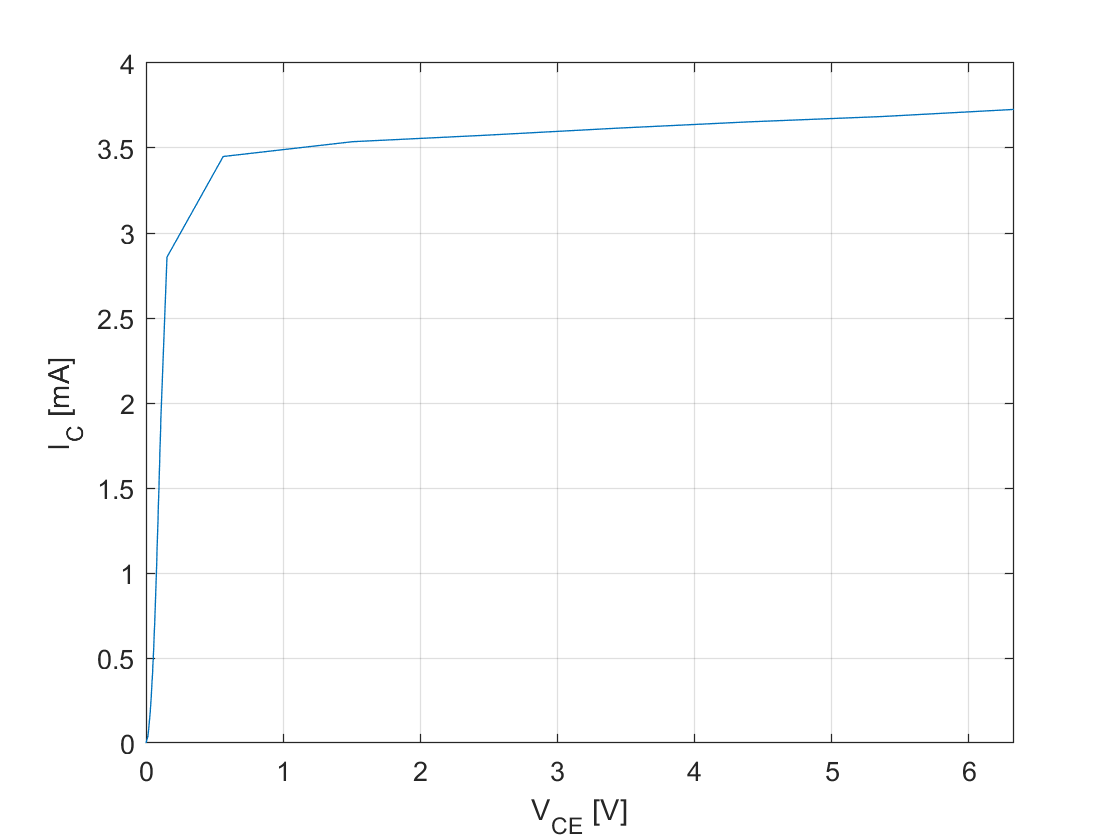
\includegraphics[scale=0.4]{./images/bjt_ic_vce.PNG}
	\caption{BJT $I_C$ versus $V_{CE}$ Plot}
	\label{fig:bjt_ic_vce}
\end{figure}

\FloatBarrier

The $I_C - V_{BE}$ curve from the measured values above again exhibit the expected behavior. The BJT is observed to in the saturation region when $V_{CE}$ is less than approximately 0.6V and $I_C$ is observed to saturate at approximately 3.5mA and the active region is then observed. 
